\documentclass{article}
\usepackage[utf8]{inputenc}
\usepackage[T1]{fontenc}
\usepackage{graphicx}
\usepackage{algorithm}
\usepackage{algpseudocode}

\usepackage{listings}
\usepackage{xcolor}
\usepackage[margin=2.5cm]{geometry}
\usepackage{float}

\usepackage{amssymb} %Ajoute des symboles mathématiques comme R, Z, forall, exists, etc....
\usepackage{amsmath}
\usepackage{amsthm}


\lstdefinestyle{monstyle}{
    backgroundcolor=\color{white},
    commentstyle=\color{gray},
    keywordstyle=\color{blue},
    numberstyle=\tiny\color{gray},
    basicstyle=\ttfamily\small,
    breaklines=true,
    numbers=left,
    numbersep=5pt,
    frame=single,
}
\lstset{style=monstyle}

\title{\textbf{Rapport TD n°2 : Initiation à l'algorithmique}}
\author{Derrez Lorenzo}

\begin{document}
\maketitle

\section*{Exercice 1}
\subsection*{Question 1}

\begin{itemize}
    \item On a pour le premier tableau : 
    \subitem T = a(T)
    \subitem a(T)
    \subitem b(T)
    \item Les trois propositions sont par ailleurs équivalentes 
\end{itemize}
\subsection*{Question 2}

\begin{itemize}
    \item On a pour le deuxième tableau : 
    \subitem a(T); a(T)
    \subitem b(T); b(T)
    \subitem a(a(T))
    \subitem b(a(T))
    \item Les quatre propositions sont équivalentes entre elle, on préfèrerait cependant écrire b(T);b(T) par lisibilité
\end{itemize}

\section*{Exercice 2}

Voici les différents états dans lequel se trouve la pile d'appel lors de l'exécution de \textit{f} sur l'entrée 4 : 
\begin{itemize}
    \item 
\end{itemize}

\section*{Exercice 3}
Voici les différents arbres d'appels que l'on peut dessiner par rapport aux 4 fonctions : 


\begin{minipage}[c]{10cm}
    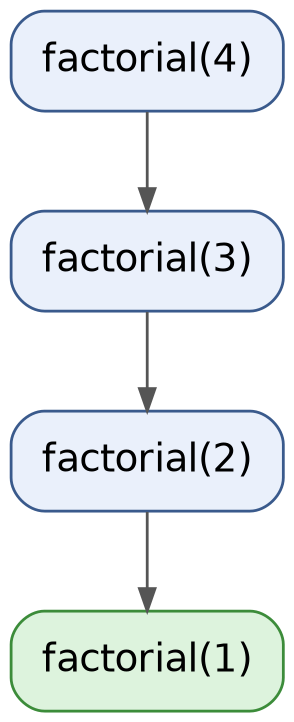
\includegraphics[width=4cm]{arbre_1_factorial.png}
\end{minipage}


\begin{minipage}[c]{10cm}
    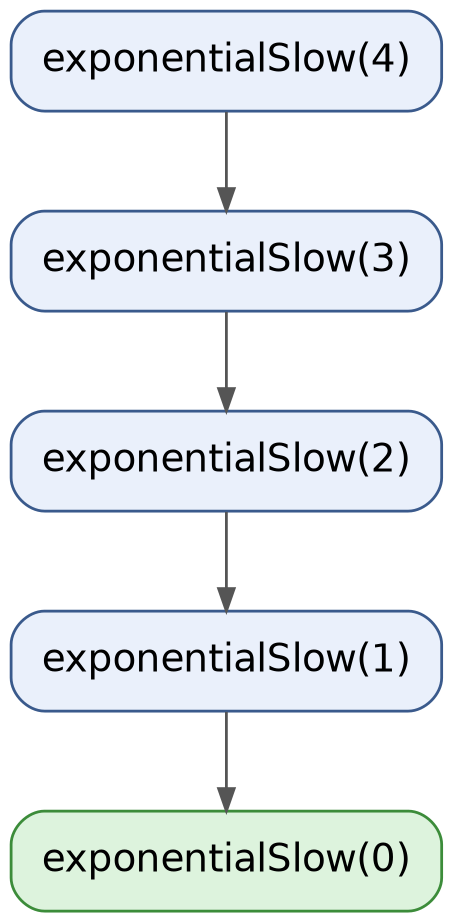
\includegraphics[width=4cm]{arbre_2_exponentialSlow.png}
\end{minipage}


\begin{minipage}[c]{20cm}
    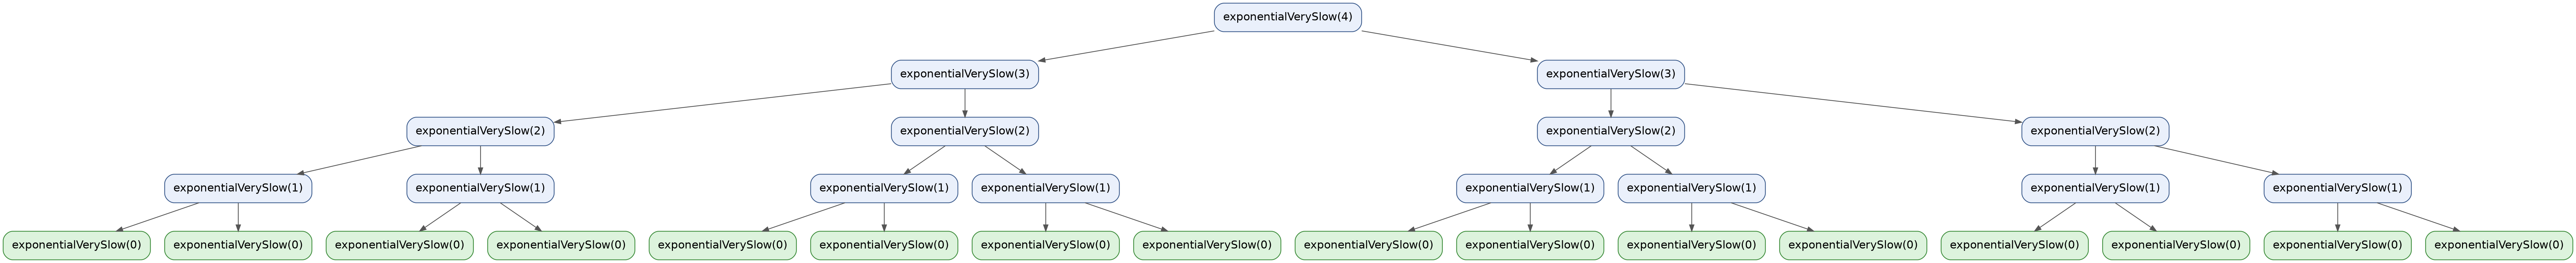
\includegraphics[width=18cm]{arbre_3_exponentialVerySlow.png}
\end{minipage}


\begin{minipage}[c]{20cm}
    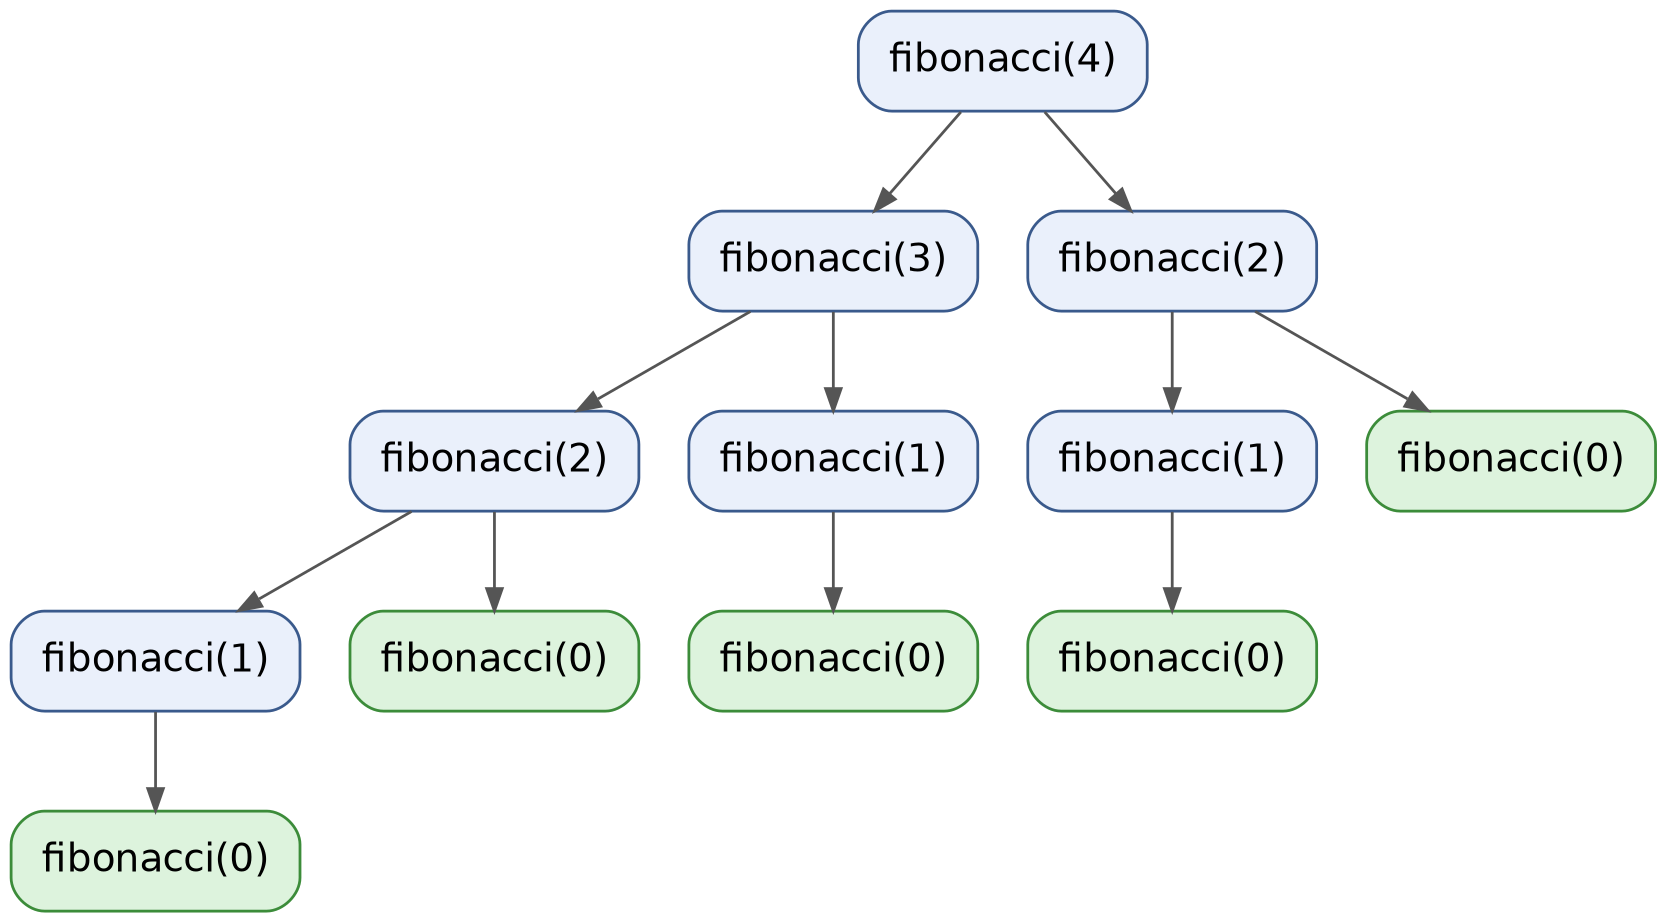
\includegraphics[width=8cm]{arbre_4_fibonacci.png}
\end{minipage}

\section*{Exercice 4}

\section*{Exercice 5}

\subsection*{Question 1 :}

On définit la proposition $\mathcal{P}(n)$ par :
$$
x^n =
\begin{cases}
1 & \text{si } n = 0 \\
x \times x^{n-1} & \text{si } n \text{ est impair} \\
\left(x^{n/2}\right)^2 & \text{si } n \text{ est pair}, \ n > 0
\end{cases}
$$

\subsection*{Question 2 :}

    \begin{algorithm}
        \caption{\textit{power}}
        \begin{algorithmic}[1]
            \State Entrée : $x \in \mathbb{Z}$, $n \in \mathbb{N}$
            \State Sortie : $ x^n $ un entier
            \Function {power}{x,n}
                \quad \State Si (n = 0) alors 
                \\
                \quad \quad \Return 1
                \\
                \quad Sinon Si (n est impair) alors
                \\ 
                \quad \quad \Return $ x * power(x, n-1) $
                \\ 
                \quad Sinon 
                \\ 
                \quad \quad \Return $ (power(x, n/2)) ^{2}$
            \EndFunction
        \end{algorithmic}
    \end{algorithm}

\subsection*{Question 3 :}


\begin{minipage}[c]{10cm}
    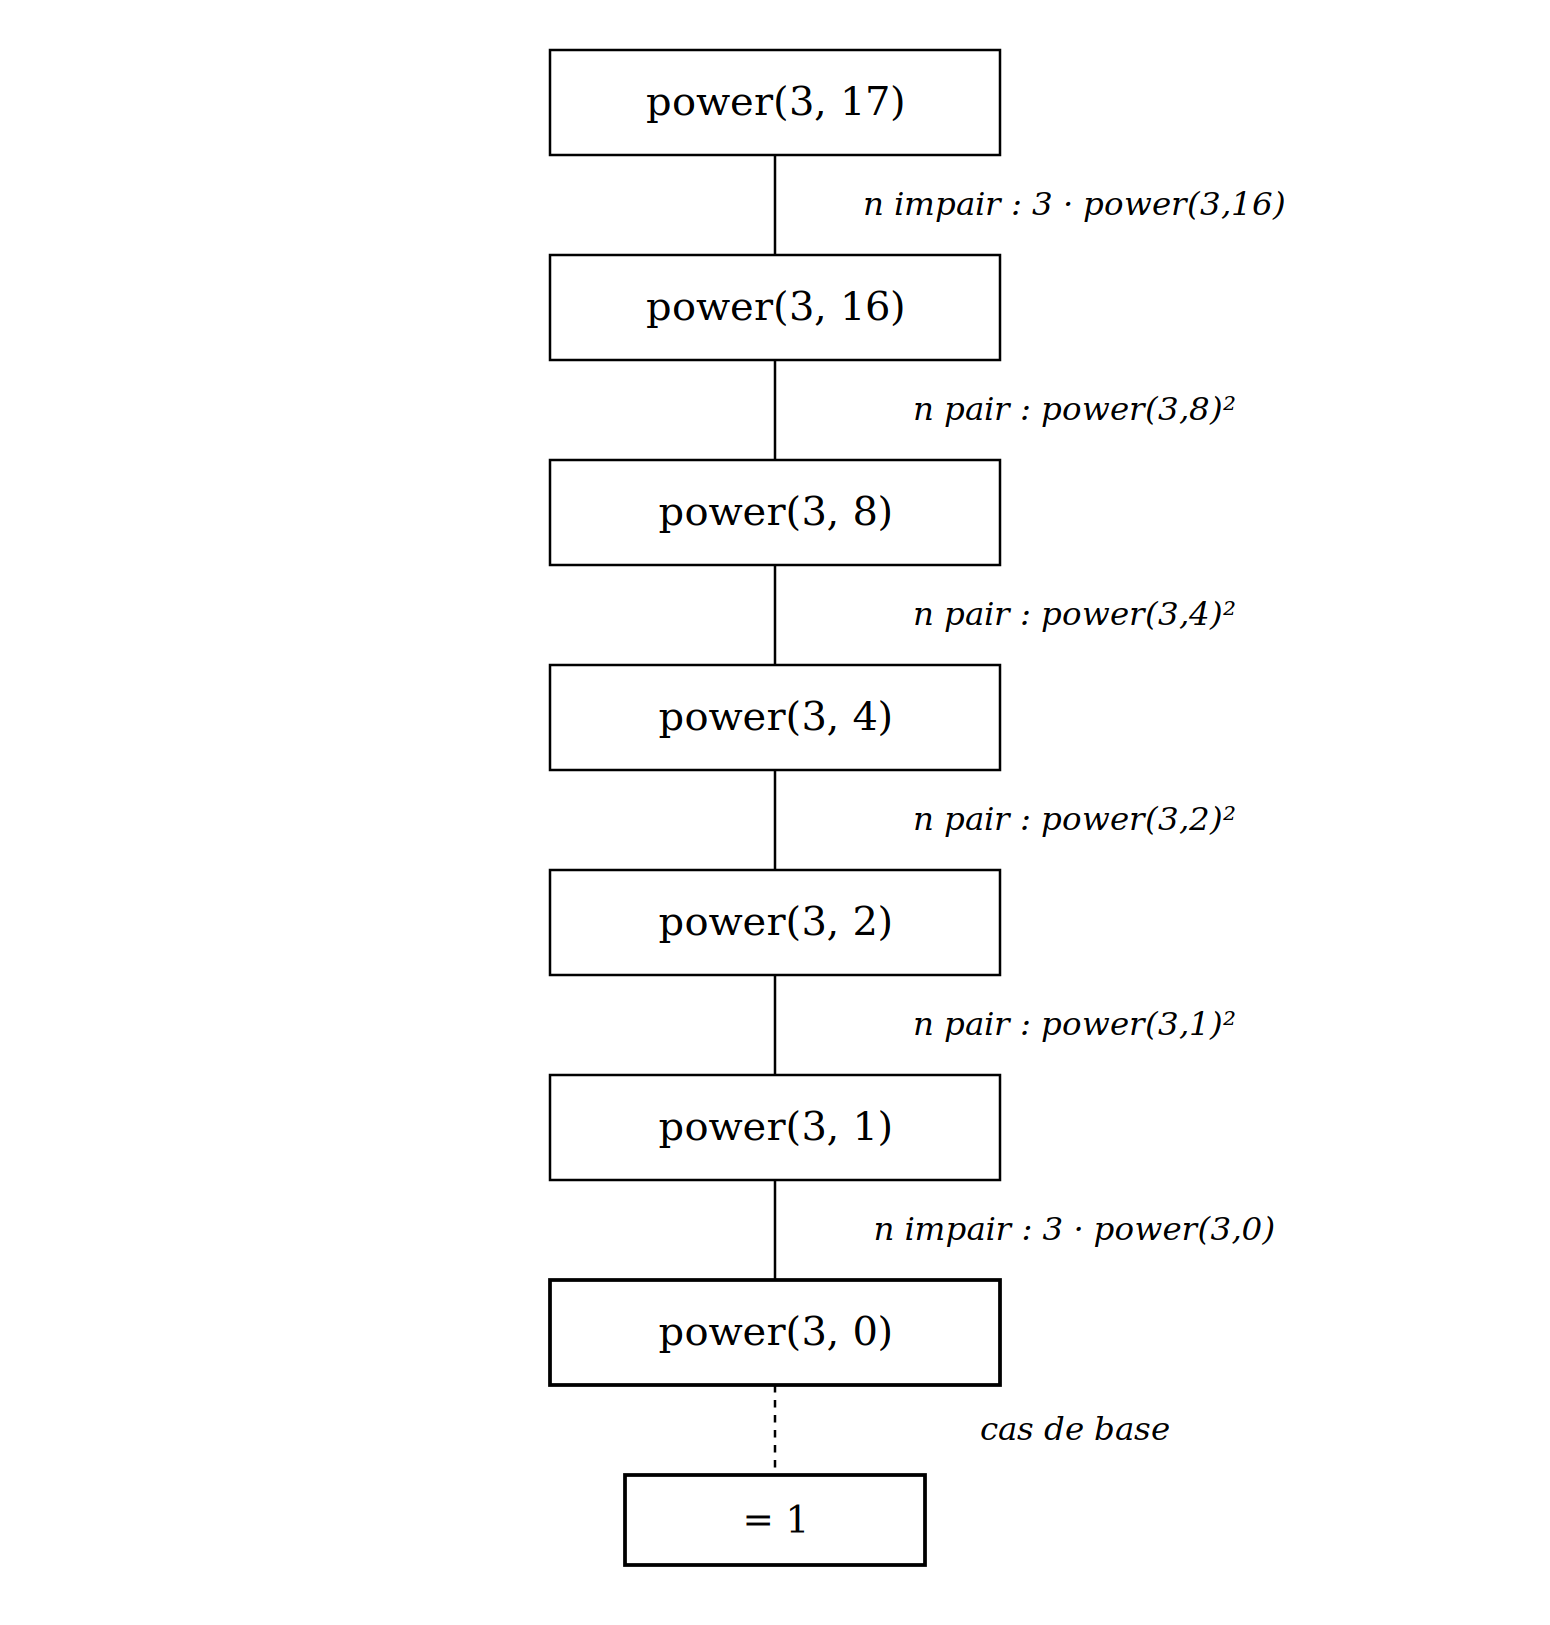
\includegraphics[width=8cm]{arbre_appels_power_3_17_minimal.png}
\end{minipage}

\subsection*{Question 4 :}

Soit $\mathcal{C}(n)$ le nombre total d'appels (avec l'appel initial), on a : 
\begin{itemize}
    \item $ \mathcal{C}(0) = 1 $ 
    \item $ \mathcal{C}(n) = \mathcal{C}(n-1)+1 \text{ si } n \text{ est impair}$
    \item $ \mathcal{C}(n) = \mathcal{C}(n/2)+1 \text{ si} n \text{ est pair} $
\end{itemize}

En comptant sur l'exemple n = 17 on obtient : \textbf{7 appels}.

\subsection*{Question 5 :}

\begin{itemize}
    \item \textbf{ExponentialSlow} effectue n+1 appels.
    \item \textbf{ExponentialVerySlow} en effectue $ 2^{n+1} -1 $
\end{itemize}

\section*{Exercice 6}

\begin{itemize}
    \item Il semblerait que la fonction \textit{Fibonnaci} se rapproche de l'écriture de la fonction \textit{ExponentialVerySlow} (Par ailleurs, cela se voit en étudiant les arbres d'appels de l'exercice 3).
    \item Effectivement, on peut réduire le nombre d'appels de la fonction \textit{Fibonacci} en utilisant le principe de \textit{programmation dynamique}.
        \subitem On ajoute en paramètre un tableau \textit{memo} qui va stocker les valeurs déjà calculées. 
\end{itemize}

\begin{algorithm}
    \caption{Fibonnaci par programmation dynamique}
    \begin{algorithmic}[1]
        \State Entrée : \textit{x} un entier, \textit{memo} un tableau d'entiers
        \State Sortie : \textit{fibo(x)} un entier
        \Function {Fibo}{\textit{x, memo}} :
            \\
            \quad $ memo[0] \leftarrow 0$
            \\
            \quad $ memo[1] \leftarrow 1$
            \\
            \quad $ int~i \leftarrow 2$
            \\
            \quad Tant que (i<=n) faire :
            \\
            \quad \quad $ memo[i] \leftarrow {memo[i-1] + memo[i-2]}$
            \\
            \quad \quad $ i \leftarrow {i + 1}$
            \\
            \quad \Return memo[x]
        \EndFunction
    \end{algorithmic}
\end{algorithm}

\end{document}